% !TEX root = ./MParticle_resubmit.tex
\section{Numerical Implementation}
A cycle-based max pressure controller was implemented on a network of 11 signalized intersections modeled in Aimsun, a micro-simulation platform commonly used by practitioners. The present simulation was generated as part of the I-15 Integrated Corridor Management project undertaken by the San Diego Association of Governments in San Diego, CA. 
The cycle-based controller was set to run with a cycle length of 90 seconds and minimum time constraints of 10 seconds for each of the 3-4 available standard signal control stages.  
\begin{figure}[h!]
\vspace{-.2em}
\centering
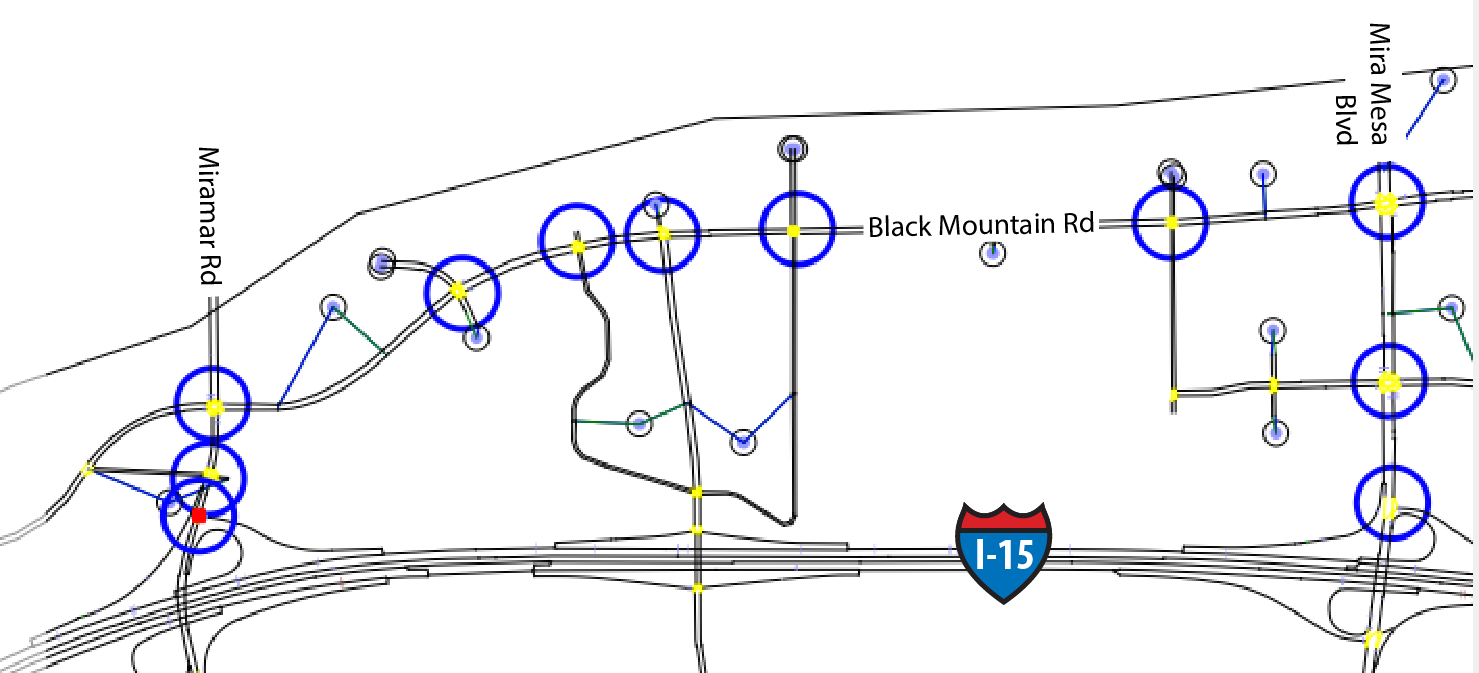
\includegraphics[width=.8\columnwidth]{./i15network.png}
\caption{The chosen network was calibrated to represent realistic demands and physical parameters observed on a stretch of Black Mountain Road near the I-15 freeway in San Diego, California.}
\end{figure}

The remainder of this section provides a comparison of the performance of the cycle-based max pressure algorithm with two other control algorithms described below. While it makes sense to compare the numerical performance of these algorithms, it should be noted that while the other algorithms seem to perform well in simulation, they come with no proof or theoretical guarantees on operation.
 
Various performance metrics were compared between model runs using the max pressure controller and two alternative controllers: a fixed-time control plan that divides each signal cycle equally between all available phases, and a ``fully-actuated'' control system such as that which is currently operational on the real road network represented by the model. The fully actuated-controller is essentially a flexible fixed-time plan in which green times can be shortened or extended in real time to promote continuity of flows in response to instantaneous link demand measurements. 
%\begin{figure}[h!]
%\centering
%\includegraphics[width=\columnwidth]{./AIMSUN_intersection.png}
%\caption{Cycle-allocated max pressure was implemented using a cycle length of 90 seconds and minimum time constraints of 10 seconds for each phase.}
%\end{figure}
The comparison of network vehicle counts in Figure \ref{fig_counts} suggests that the uniformly-allocated fixed time controller caused significantly fewer vehicles to be served than the other two controllers, which were comparable to each other in vehicle service rates. This difference made it difficult to fairly compare other performance metrics between the uniform fixed-time controller and the other two options. 
\begin{figure}[h!]
\centering
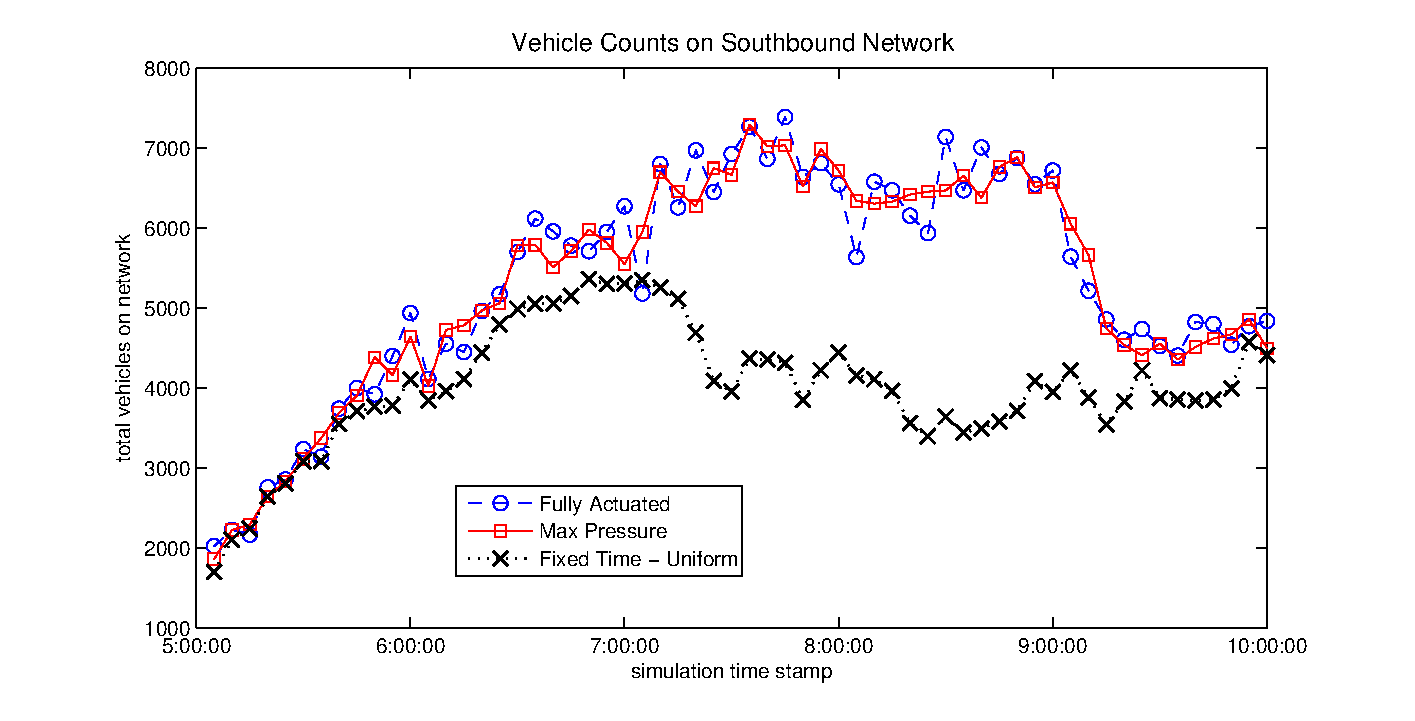
\includegraphics[width=\columnwidth]{./VehicleCountsPlot.eps}
\vspace{-2em}
\caption{During congestion, cycle-based max pressure demonstrated service rates that are higher than the uniformly allocated fixed-time controller and consistent with a fully-actuated control system.  \label{fig_counts}}
\end{figure}
\begin{figure}[h!]
\vspace{-.5em}
\centering
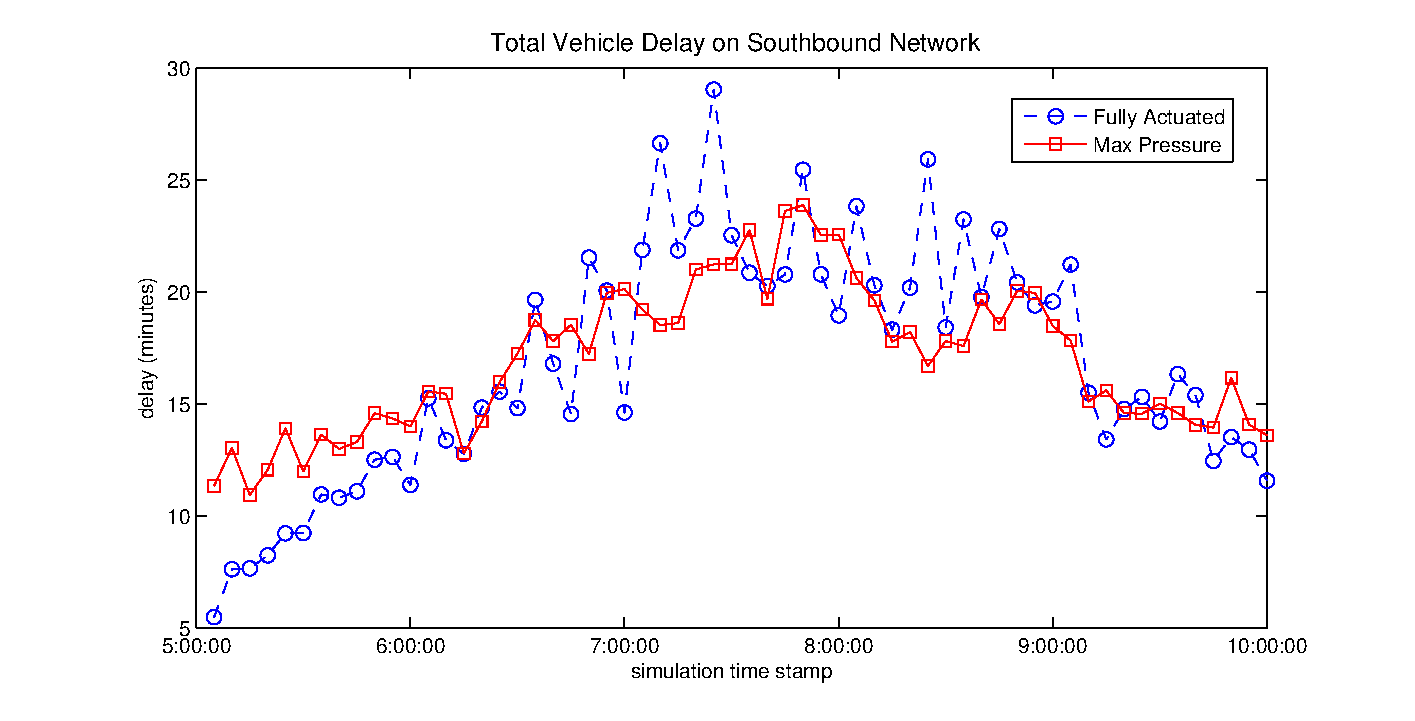
\includegraphics[width=\columnwidth]{./VehicleDelayPlot.eps}
\vspace{-2em}
\caption{Max pressure outperforms the fully actuated system during periods of high demand.\label{fig_delay}}
\vspace{-1em}
\end{figure}

Differences between the fully-actuated and cycle-based max pressure controllers were observed in measurements of delays and queue lengths: while the fully-actuated system appeared to produce less delay and shorter queues than max pressure during periods of relatively low network demand, max pressure was equally as effective or even more effective at reducing delays and queue lengths given larger demands. Figure \ref{fig_delay} shows how delays were reduced and had less variance over time when the max pressure controller was applied than with the fully-actuated controller. 
\begin{figure}[h!]
\centering
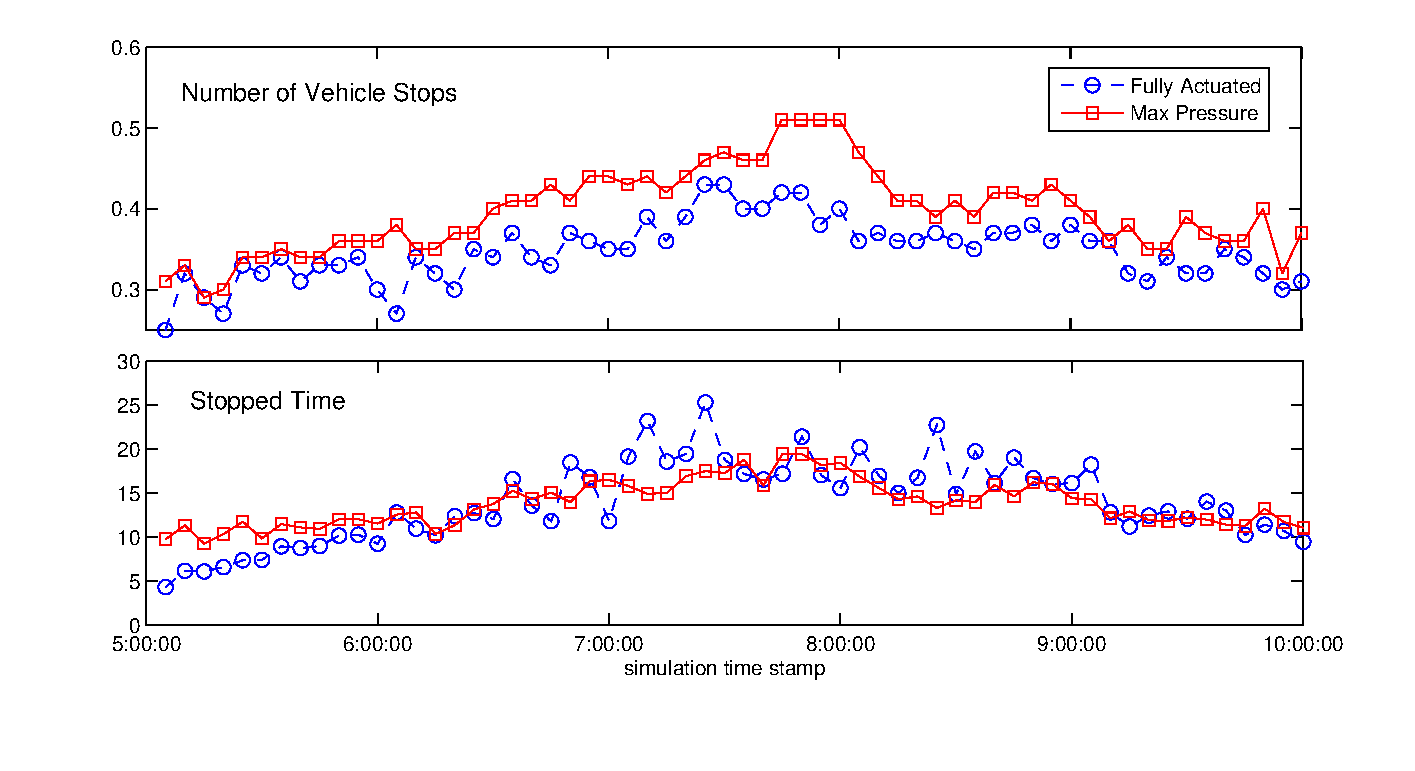
\includegraphics[width=\columnwidth]{./VehicleStopsPlot.eps}
\vspace{-2.5em}
\caption{While max pressure caused more vehicle stop events, stoppage times were similar to those observed using the standard fully-actuated controller.\label{fig_stops}}
\end{figure}

Cycle-based max pressure consistently induced more stops during a vehicle's journey across the network, which is expected given the design objectives of the fully-actuated system. As illustrated in Figure \ref{fig_stops}, total stoppage times were higher with max pressure given low demand, but improved over the existing controller during peak demand. 

